\documentclass[1p]{elsarticle_modified}
%\bibliographystyle{elsarticle-num}

%\usepackage[colorlinks]{hyperref}
%\usepackage{abbrmath_seonhwa} %\Abb, \Ascr, \Acal ,\Abf, \Afrak
\usepackage{amsfonts}
\usepackage{amssymb}
\usepackage{amsmath}
\usepackage{amsthm}
\usepackage{scalefnt}
\usepackage{amsbsy}
\usepackage{kotex}
\usepackage{caption}
\usepackage{subfig}
\usepackage{color}
\usepackage{graphicx}
\usepackage{xcolor} %% white, black, red, green, blue, cyan, magenta, yellow
\usepackage{float}
\usepackage{setspace}
\usepackage{hyperref}

\usepackage{tikz}
\usetikzlibrary{arrows}

\usepackage{multirow}
\usepackage{array} % fixed length table
\usepackage{hhline}

%%%%%%%%%%%%%%%%%%%%%
\makeatletter
\renewcommand*\env@matrix[1][\arraystretch]{%
	\edef\arraystretch{#1}%
	\hskip -\arraycolsep
	\let\@ifnextchar\new@ifnextchar
	\array{*\c@MaxMatrixCols c}}
\makeatother %https://tex.stackexchange.com/questions/14071/how-can-i-increase-the-line-spacing-in-a-matrix
%%%%%%%%%%%%%%%

\usepackage[normalem]{ulem}

\newcommand{\msout}[1]{\ifmmode\text{\sout{\ensuremath{#1}}}\else\sout{#1}\fi}
%SOURCE: \msout is \stkout macro in https://tex.stackexchange.com/questions/20609/strikeout-in-math-mode

\newcommand{\cancel}[1]{
	\ifmmode
	{\color{red}\msout{#1}}
	\else
	{\color{red}\sout{#1}}
	\fi
}

\newcommand{\add}[1]{
	{\color{blue}\uwave{#1}}
}

\newcommand{\replace}[2]{
	\ifmmode
	{\color{red}\msout{#1}}{\color{blue}\uwave{#2}}
	\else
	{\color{red}\sout{#1}}{\color{blue}\uwave{#2}}
	\fi
}

\newcommand{\Sol}{\mathcal{S}} %segment
\newcommand{\D}{D} %diagram
\newcommand{\A}{\mathcal{A}} %arc


%%%%%%%%%%%%%%%%%%%%%%%%%%%%%5 test

\def\sl{\operatorname{\textup{SL}}(2,\Cbb)}
\def\psl{\operatorname{\textup{PSL}}(2,\Cbb)}
\def\quan{\mkern 1mu \triangleright \mkern 1mu}

\theoremstyle{definition}
\newtheorem{thm}{Theorem}[section]
\newtheorem{prop}[thm]{Proposition}
\newtheorem{lem}[thm]{Lemma}
\newtheorem{ques}[thm]{Question}
\newtheorem{cor}[thm]{Corollary}
\newtheorem{defn}[thm]{Definition}
\newtheorem{exam}[thm]{Example}
\newtheorem{rmk}[thm]{Remark}
\newtheorem{alg}[thm]{Algorithm}

\newcommand{\I}{\sqrt{-1}}
\begin{document}

%\begin{frontmatter}
%
%\title{Boundary parabolic representations of knots up to 8 crossings}
%
%%% Group authors per affiliation:
%\author{Yunhi Cho} 
%\address{Department of Mathematics, University of Seoul, Seoul, Korea}
%\ead{yhcho@uos.ac.kr}
%
%
%\author{Seonhwa Kim} %\fnref{s_kim}}
%\address{Center for Geometry and Physics, Institute for Basic Science, Pohang, 37673, Korea}
%\ead{ryeona17@ibs.re.kr}
%
%\author{Hyuk Kim}
%\address{Department of Mathematical Sciences, Seoul National University, Seoul 08826, Korea}
%\ead{hyukkim@snu.ac.kr}
%
%\author{Seokbeom Yoon}
%\address{Department of Mathematical Sciences, Seoul National University, Seoul, 08826,  Korea}
%\ead{sbyoon15@snu.ac.kr}
%
%\begin{abstract}
%We find all boundary parabolic representation of knots up to 8 crossings.
%
%\end{abstract}
%\begin{keyword}
%    \MSC[2010] 57M25 
%\end{keyword}
%
%\end{frontmatter}

%\linenumbers
%\tableofcontents
%
\newcommand\colored[1]{\textcolor{white}{\rule[-0.35ex]{0.8em}{1.4ex}}\kern-0.8em\color{red} #1}%
%\newcommand\colored[1]{\textcolor{white}{ #1}\kern-2.17ex	\textcolor{white}{ #1}\kern-1.81ex	\textcolor{white}{ #1}\kern-2.15ex\color{red}#1	}

{\Large $\underline{12a_{0009}~(K12a_{0009})}$}

\setlength{\tabcolsep}{10pt}
\renewcommand{\arraystretch}{1.6}
\vspace{1cm}\begin{tabular}{m{100pt}>{\centering\arraybackslash}m{274pt}}
\multirow{5}{120pt}{
	\centering
	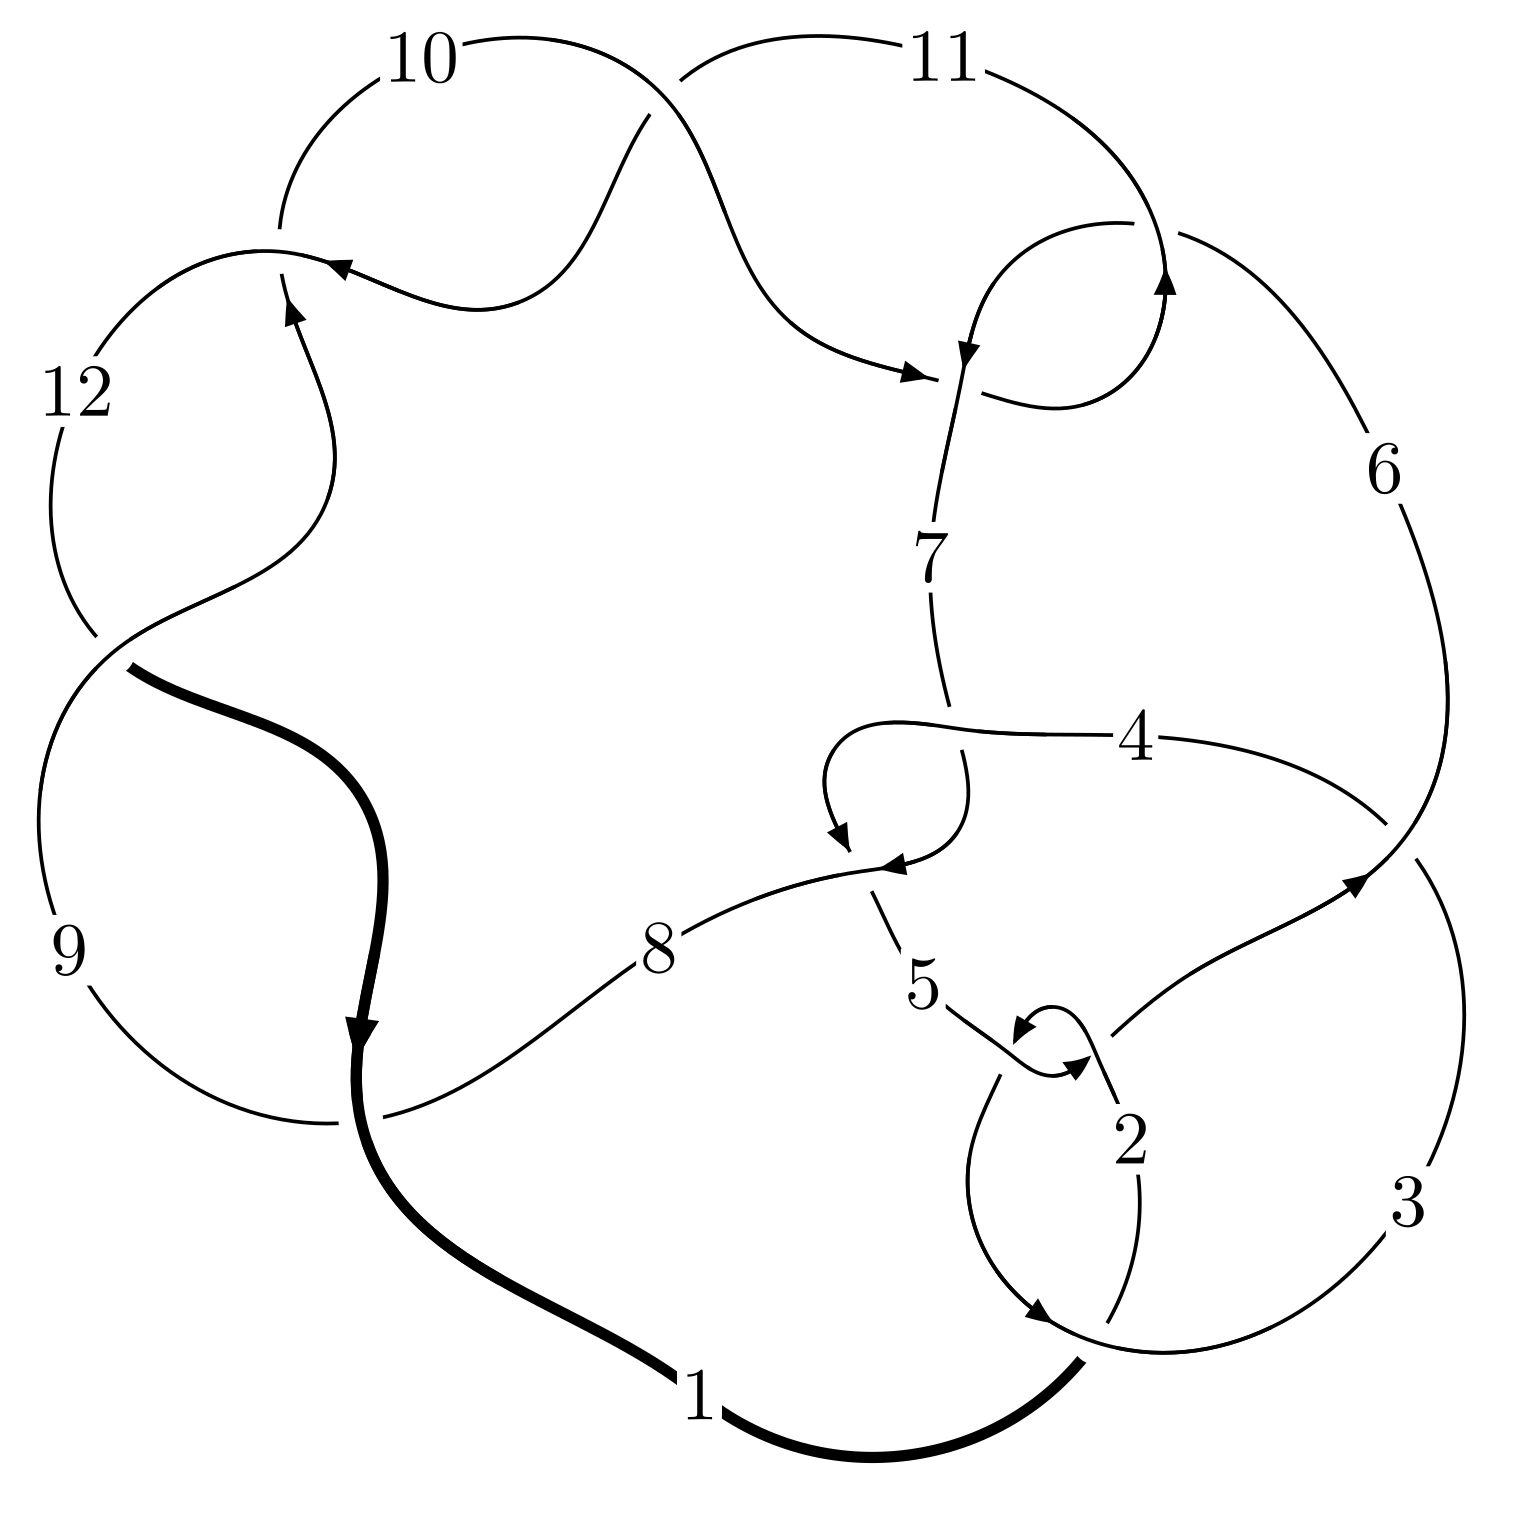
\includegraphics[width=112pt]{../../../GIT/diagram.site/Diagrams/png/810_12a_0009.png}\\
\ \ \ A knot diagram\footnotemark}&
\allowdisplaybreaks
\textbf{Linearized knot diagam} \\
\cline{2-2}
 &
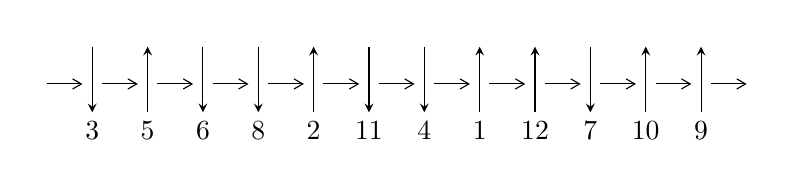
\begin{tikzpicture}[x=20pt, y=17pt]
	% nodes
	\node (C0) at (0, 0) {};
	\node (C1) at (1, 0) {};
	\node (C1U) at (1, +1) {};
	\node (C1D) at (1, -1) {3};

	\node (C2) at (2, 0) {};
	\node (C2U) at (2, +1) {};
	\node (C2D) at (2, -1) {5};

	\node (C3) at (3, 0) {};
	\node (C3U) at (3, +1) {};
	\node (C3D) at (3, -1) {6};

	\node (C4) at (4, 0) {};
	\node (C4U) at (4, +1) {};
	\node (C4D) at (4, -1) {8};

	\node (C5) at (5, 0) {};
	\node (C5U) at (5, +1) {};
	\node (C5D) at (5, -1) {2};

	\node (C6) at (6, 0) {};
	\node (C6U) at (6, +1) {};
	\node (C6D) at (6, -1) {11};

	\node (C7) at (7, 0) {};
	\node (C7U) at (7, +1) {};
	\node (C7D) at (7, -1) {4};

	\node (C8) at (8, 0) {};
	\node (C8U) at (8, +1) {};
	\node (C8D) at (8, -1) {1};

	\node (C9) at (9, 0) {};
	\node (C9U) at (9, +1) {};
	\node (C9D) at (9, -1) {12};

	\node (C10) at (10, 0) {};
	\node (C10U) at (10, +1) {};
	\node (C10D) at (10, -1) {7};

	\node (C11) at (11, 0) {};
	\node (C11U) at (11, +1) {};
	\node (C11D) at (11, -1) {10};

	\node (C12) at (12, 0) {};
	\node (C12U) at (12, +1) {};
	\node (C12D) at (12, -1) {9};
	\node (C13) at (13, 0) {};

	% arrows
	\draw[->,>={angle 60}]
	(C0) edge (C1) (C1) edge (C2) (C2) edge (C3) (C3) edge (C4) (C4) edge (C5) (C5) edge (C6) (C6) edge (C7) (C7) edge (C8) (C8) edge (C9) (C9) edge (C10) (C10) edge (C11) (C11) edge (C12) (C12) edge (C13) ;	\draw[->,>=stealth]
	(C1U) edge (C1D) (C2D) edge (C2U) (C3U) edge (C3D) (C4U) edge (C4D) (C5D) edge (C5U) (C6U) edge (C6D) (C7U) edge (C7D) (C8D) edge (C8U) (C9D) edge (C9U) (C10U) edge (C10D) (C11D) edge (C11U) (C12D) edge (C12U) ;
	\end{tikzpicture} \\
\hhline{~~} \\& 
\textbf{Solving Sequence} \\ \cline{2-2} 
 &
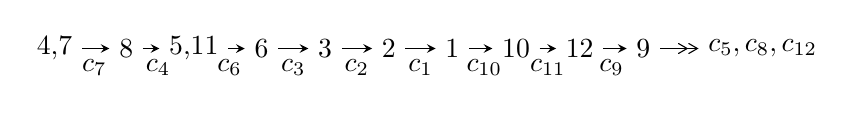
\begin{tikzpicture}[x=23pt, y=7pt]
	% node
	\node (A0) at (-1/8, 0) {4,7};
	\node (A1) at (1, 0) {8};
	\node (A2) at (33/16, 0) {5,11};
	\node (A3) at (25/8, 0) {6};
	\node (A4) at (33/8, 0) {3};
	\node (A5) at (41/8, 0) {2};
	\node (A6) at (49/8, 0) {1};
	\node (A7) at (57/8, 0) {10};
	\node (A8) at (65/8, 0) {12};
	\node (A9) at (73/8, 0) {9};
	\node (C1) at (1/2, -1) {$c_{7}$};
	\node (C2) at (3/2, -1) {$c_{4}$};
	\node (C3) at (21/8, -1) {$c_{6}$};
	\node (C4) at (29/8, -1) {$c_{3}$};
	\node (C5) at (37/8, -1) {$c_{2}$};
	\node (C6) at (45/8, -1) {$c_{1}$};
	\node (C7) at (53/8, -1) {$c_{10}$};
	\node (C8) at (61/8, -1) {$c_{11}$};
	\node (C9) at (69/8, -1) {$c_{9}$};
	\node (A10) at (11, 0) {$c_{5},c_{8},c_{12}$};

	% edge
	\draw[->,>=stealth]	
	(A0) edge (A1) (A1) edge (A2) (A2) edge (A3) (A3) edge (A4) (A4) edge (A5) (A5) edge (A6) (A6) edge (A7) (A7) edge (A8) (A8) edge (A9) ;
	\draw[->>,>={angle 60}]	
	(A9) edge (A10);
\end{tikzpicture} \\ 

\end{tabular} \\

\footnotetext{
The image of knot diagram is generated by the software ``\textbf{Draw programme}" developed by Andrew Bartholomew(\url{http://www.layer8.co.uk/maths/draw/index.htm\#Running-draw}), where we modified some parts for our purpose(\url{https://github.com/CATsTAILs/LinksPainter}).
}\phantom \\ \newline 
\centering \textbf{Ideals for irreducible components\footnotemark of $X_{\text{par}}$} 
 
\begin{align*}
I^u_{1}&=\langle 
1.86386\times10^{139} u^{66}+4.31229\times10^{138} u^{65}+\cdots+1.98538\times10^{140} b+5.26231\times10^{141},\\
\phantom{I^u_{1}}&\phantom{= \langle  }1.05918\times10^{140} u^{66}-4.57520\times10^{138} u^{65}+\cdots+7.94151\times10^{140} a+2.63032\times10^{142},\\
\phantom{I^u_{1}}&\phantom{= \langle  }u^{67}+u^{66}+\cdots+384 u+256\rangle \\
\\
I^v_{1}&=\langle 
a,\;18 v^7-26 v^6+12 v^5-78 v^4+71 v^3+30 v^2+19 b+6 v-2,\;v^8-2 v^7+v^6-4 v^5+6 v^4+v^3-2 v^2- v+1\rangle \\
\end{align*}
\raggedright * 2 irreducible components of $\dim_{\mathbb{C}}=0$, with total 75 representations.\\
\footnotetext{All coefficients of polynomials are rational numbers. But the coefficients are sometimes approximated in decimal forms when there is not enough margin.}
\newpage
\renewcommand{\arraystretch}{1}
\centering \section*{I. $I^u_{1}= \langle 1.86\times10^{139} u^{66}+4.31\times10^{138} u^{65}+\cdots+1.99\times10^{140} b+5.26\times10^{141},\;1.06\times10^{140} u^{66}-4.58\times10^{138} u^{65}+\cdots+7.94\times10^{140} a+2.63\times10^{142},\;u^{67}+u^{66}+\cdots+384 u+256 \rangle$}
\flushleft \textbf{(i) Arc colorings}\\
\begin{tabular}{m{7pt} m{180pt} m{7pt} m{180pt} }
\flushright $a_{4}=$&$\begin{pmatrix}0\\u\end{pmatrix}$ \\
\flushright $a_{7}=$&$\begin{pmatrix}1\\0\end{pmatrix}$ \\
\flushright $a_{8}=$&$\begin{pmatrix}1\\u^2\end{pmatrix}$ \\
\flushright $a_{5}=$&$\begin{pmatrix}- u\\- u^3+u\end{pmatrix}$ \\
\flushright $a_{11}=$&$\begin{pmatrix}-0.133372 u^{66}+0.00576112 u^{65}+\cdots-11.7330 u-33.1212\\-0.0938796 u^{66}-0.0217203 u^{65}+\cdots-6.32205 u-26.5053\end{pmatrix}$ \\
\flushright $a_{6}=$&$\begin{pmatrix}0.209669 u^{66}+0.0230614 u^{65}+\cdots+21.6013 u+63.8657\\-0.0241755 u^{66}+0.0237769 u^{65}+\cdots-9.20588 u-1.31583\end{pmatrix}$ \\
\flushright $a_{3}=$&$\begin{pmatrix}-0.142701 u^{66}-0.0190334 u^{65}+\cdots-17.1447 u-45.4624\\-0.0396775 u^{66}-0.0112029 u^{65}+\cdots-1.07906 u-14.6917\end{pmatrix}$ \\
\flushright $a_{2}=$&$\begin{pmatrix}-0.111576 u^{66}+0.000157764 u^{65}+\cdots-14.6284 u-30.1716\\-0.0827762 u^{66}-0.0101687 u^{65}+\cdots-6.98086 u-26.9277\end{pmatrix}$ \\
\flushright $a_{1}=$&$\begin{pmatrix}-0.185494 u^{66}-0.0468383 u^{65}+\cdots-12.3954 u-62.5498\\-0.120165 u^{66}-0.00728459 u^{65}+\cdots-14.9632 u-36.8117\end{pmatrix}$ \\
\flushright $a_{10}=$&$\begin{pmatrix}-0.227252 u^{66}-0.0159592 u^{65}+\cdots-18.0550 u-59.6265\\-0.0938796 u^{66}-0.0217203 u^{65}+\cdots-6.32205 u-26.5053\end{pmatrix}$ \\
\flushright $a_{12}=$&$\begin{pmatrix}-0.280258 u^{66}-0.0158075 u^{65}+\cdots-25.1937 u-78.0193\\-0.194157 u^{66}-0.0107796 u^{65}+\cdots-23.6385 u-52.3816\end{pmatrix}$ \\
\flushright $a_{9}=$&$\begin{pmatrix}-0.0947524 u^{66}-0.0190567 u^{65}+\cdots-3.59061 u-27.7303\\-0.0296424 u^{66}-0.00314345 u^{65}+\cdots-7.50843 u-12.6063\end{pmatrix}$\\&\end{tabular}
\flushleft \textbf{(ii) Obstruction class $= -1$}\\~\\
\flushleft \textbf{(iii) Cusp Shapes $= -0.257514 u^{66}+0.0210201 u^{65}+\cdots-47.1768 u-88.2413$}\\~\\
\newpage\renewcommand{\arraystretch}{1}
\flushleft \textbf{(iv) u-Polynomials at the component}\newline \\
\begin{tabular}{m{50pt}|m{274pt}}
Crossings & \hspace{64pt}u-Polynomials at each crossing \\
\hline $$\begin{aligned}c_{1}\end{aligned}$$&$\begin{aligned}
&u^{67}+35 u^{66}+\cdots-6 u-1
\end{aligned}$\\
\hline $$\begin{aligned}c_{2},c_{5}\end{aligned}$$&$\begin{aligned}
&u^{67}+5 u^{66}+\cdots+4 u+1
\end{aligned}$\\
\hline $$\begin{aligned}c_{3}\end{aligned}$$&$\begin{aligned}
&u^{67}-5 u^{66}+\cdots-4396 u+833
\end{aligned}$\\
\hline $$\begin{aligned}c_{4},c_{7}\end{aligned}$$&$\begin{aligned}
&u^{67}+u^{66}+\cdots+384 u+256
\end{aligned}$\\
\hline $$\begin{aligned}c_{6},c_{10}\end{aligned}$$&$\begin{aligned}
&u^{67}+3 u^{66}+\cdots+3 u^2+1
\end{aligned}$\\
\hline $$\begin{aligned}c_{8},c_{9},c_{11}\\c_{12}\end{aligned}$$&$\begin{aligned}
&u^{67}-13 u^{66}+\cdots-6 u+1
\end{aligned}$\\
\hline
\end{tabular}\\~\\
\newpage\renewcommand{\arraystretch}{1}
\flushleft \textbf{(v) Riley Polynomials at the component}\newline \\
\begin{tabular}{m{50pt}|m{274pt}}
Crossings & \hspace{64pt}Riley Polynomials at each crossing \\
\hline $$\begin{aligned}c_{1}\end{aligned}$$&$\begin{aligned}
&y^{67}- y^{66}+\cdots+26 y-1
\end{aligned}$\\
\hline $$\begin{aligned}c_{2},c_{5}\end{aligned}$$&$\begin{aligned}
&y^{67}+35 y^{66}+\cdots-6 y-1
\end{aligned}$\\
\hline $$\begin{aligned}c_{3}\end{aligned}$$&$\begin{aligned}
&y^{67}-37 y^{66}+\cdots-10001782 y-693889
\end{aligned}$\\
\hline $$\begin{aligned}c_{4},c_{7}\end{aligned}$$&$\begin{aligned}
&y^{67}-45 y^{66}+\cdots+770048 y-65536
\end{aligned}$\\
\hline $$\begin{aligned}c_{6},c_{10}\end{aligned}$$&$\begin{aligned}
&y^{67}+13 y^{66}+\cdots-6 y-1
\end{aligned}$\\
\hline $$\begin{aligned}c_{8},c_{9},c_{11}\\c_{12}\end{aligned}$$&$\begin{aligned}
&y^{67}+85 y^{66}+\cdots-214 y-1
\end{aligned}$\\
\hline
\end{tabular}\\~\\
\newpage\flushleft \textbf{(vi) Complex Volumes and Cusp Shapes}
$$\begin{array}{c|c|c}  
\text{Solutions to }I^u_{1}& \I (\text{vol} + \sqrt{-1}CS) & \text{Cusp shape}\\
 \hline 
\begin{aligned}
u &= \phantom{-}0.056677 + 1.011830 I \\
a &= \phantom{-}0.252444 + 1.241020 I \\
b &= -0.625082 - 0.683742 I\end{aligned}
 & -2.90819 + 1.25830 I & -6.22598 - 0.52297 I \\ \hline\begin{aligned}
u &= \phantom{-}0.056677 - 1.011830 I \\
a &= \phantom{-}0.252444 - 1.241020 I \\
b &= -0.625082 + 0.683742 I\end{aligned}
 & -2.90819 - 1.25830 I & -6.22598 + 0.52297 I \\ \hline\begin{aligned}
u &= \phantom{-}0.906722 + 0.307406 I \\
a &= -0.59144 + 2.02468 I \\
b &= -0.162929 - 0.884018 I\end{aligned}
 & \phantom{-}1.04581 - 2.21513 I & \phantom{-}3.46945 + 4.65316 I \\ \hline\begin{aligned}
u &= \phantom{-}0.906722 - 0.307406 I \\
a &= -0.59144 - 2.02468 I \\
b &= -0.162929 + 0.884018 I\end{aligned}
 & \phantom{-}1.04581 + 2.21513 I & \phantom{-}3.46945 - 4.65316 I \\ \hline\begin{aligned}
u &= -0.259205 + 1.013680 I \\
a &= \phantom{-}0.20161 + 1.64344 I \\
b &= -0.585248 - 0.823431 I\end{aligned}
 & -2.45553 - 5.81631 I & -4.24111 + 7.61398 I \\ \hline\begin{aligned}
u &= -0.259205 - 1.013680 I \\
a &= \phantom{-}0.20161 - 1.64344 I \\
b &= -0.585248 + 0.823431 I\end{aligned}
 & -2.45553 + 5.81631 I & -4.24111 - 7.61398 I \\ \hline\begin{aligned}
u &= -1.05818\phantom{ +0.000000I} \\
a &= -0.130055\phantom{ +0.000000I} \\
b &= -0.564378\phantom{ +0.000000I}\end{aligned}
 & -1.77256\phantom{ +0.000000I} & -5.82730\phantom{ +0.000000I} \\ \hline\begin{aligned}
u &= \phantom{-}0.024549 + 1.103900 I \\
a &= \phantom{-}0.011764 + 1.076850 I \\
b &= \phantom{-}0.892018 - 0.929882 I\end{aligned}
 & -8.60500 + 3.29350 I & \phantom{-0.000000 } 0 \\ \hline\begin{aligned}
u &= \phantom{-}0.024549 - 1.103900 I \\
a &= \phantom{-}0.011764 - 1.076850 I \\
b &= \phantom{-}0.892018 + 0.929882 I\end{aligned}
 & -8.60500 - 3.29350 I & \phantom{-0.000000 } 0 \\ \hline\begin{aligned}
u &= \phantom{-}0.850621 + 0.246223 I \\
a &= \phantom{-}2.15946 - 0.58175 I \\
b &= \phantom{-}0.531404 + 0.791131 I\end{aligned}
 & -0.45674 - 4.58253 I & -3.79920 + 9.11658 I\\
 \hline 
 \end{array}$$\newpage$$\begin{array}{c|c|c}  
\text{Solutions to }I^u_{1}& \I (\text{vol} + \sqrt{-1}CS) & \text{Cusp shape}\\
 \hline 
\begin{aligned}
u &= \phantom{-}0.850621 - 0.246223 I \\
a &= \phantom{-}2.15946 + 0.58175 I \\
b &= \phantom{-}0.531404 - 0.791131 I\end{aligned}
 & -0.45674 + 4.58253 I & -3.79920 - 9.11658 I \\ \hline\begin{aligned}
u &= -1.117870 + 0.087817 I \\
a &= -0.34576 + 1.97594 I \\
b &= -0.269852 - 0.943591 I\end{aligned}
 & -2.13038 + 1.08941 I & \phantom{-0.000000 } 0 \\ \hline\begin{aligned}
u &= -1.117870 - 0.087817 I \\
a &= -0.34576 - 1.97594 I \\
b &= -0.269852 + 0.943591 I\end{aligned}
 & -2.13038 - 1.08941 I & \phantom{-0.000000 } 0 \\ \hline\begin{aligned}
u &= -1.168910 + 0.077988 I \\
a &= -1.115420 - 0.446467 I \\
b &= -0.898793 - 0.925547 I\end{aligned}
 & -9.32041 - 0.45884 I & \phantom{-0.000000 } 0 \\ \hline\begin{aligned}
u &= -1.168910 - 0.077988 I \\
a &= -1.115420 + 0.446467 I \\
b &= -0.898793 + 0.925547 I\end{aligned}
 & -9.32041 + 0.45884 I & \phantom{-0.000000 } 0 \\ \hline\begin{aligned}
u &= \phantom{-}1.169990 + 0.122396 I \\
a &= -1.54997 + 0.03674 I \\
b &= -0.893032 - 0.937574 I\end{aligned}
 & -9.28166 - 6.15285 I & \phantom{-0.000000 } 0 \\ \hline\begin{aligned}
u &= \phantom{-}1.169990 - 0.122396 I \\
a &= -1.54997 - 0.03674 I \\
b &= -0.893032 + 0.937574 I\end{aligned}
 & -9.28166 + 6.15285 I & \phantom{-0.000000 } 0 \\ \hline\begin{aligned}
u &= -0.801751 + 0.037628 I \\
a &= \phantom{-}1.81454 - 0.67480 I \\
b &= \phantom{-}0.533091 - 0.711518 I\end{aligned}
 & -0.726291 - 0.492318 I & -6.66330 - 1.23227 I \\ \hline\begin{aligned}
u &= -0.801751 - 0.037628 I \\
a &= \phantom{-}1.81454 + 0.67480 I \\
b &= \phantom{-}0.533091 + 0.711518 I\end{aligned}
 & -0.726291 + 0.492318 I & -6.66330 + 1.23227 I \\ \hline\begin{aligned}
u &= \phantom{-}0.565014 + 0.542577 I \\
a &= -1.22383 + 2.12227 I \\
b &= -0.010154 - 0.774344 I\end{aligned}
 & \phantom{-}2.09008 - 1.39139 I & \phantom{-}6.88883 + 3.94894 I\\
 \hline 
 \end{array}$$\newpage$$\begin{array}{c|c|c}  
\text{Solutions to }I^u_{1}& \I (\text{vol} + \sqrt{-1}CS) & \text{Cusp shape}\\
 \hline 
\begin{aligned}
u &= \phantom{-}0.565014 - 0.542577 I \\
a &= -1.22383 - 2.12227 I \\
b &= -0.010154 + 0.774344 I\end{aligned}
 & \phantom{-}2.09008 + 1.39139 I & \phantom{-}6.88883 - 3.94894 I \\ \hline\begin{aligned}
u &= -1.166070 + 0.351089 I \\
a &= -0.46834 - 2.13436 I \\
b &= -0.162727 + 0.958944 I\end{aligned}
 & -1.53806 + 6.56529 I & \phantom{-0.000000 } 0 \\ \hline\begin{aligned}
u &= -1.166070 - 0.351089 I \\
a &= -0.46834 + 2.13436 I \\
b &= -0.162727 - 0.958944 I\end{aligned}
 & -1.53806 - 6.56529 I & \phantom{-0.000000 } 0 \\ \hline\begin{aligned}
u &= \phantom{-}0.209708 + 0.728648 I \\
a &= -0.02695 - 1.51557 I \\
b &= -0.495464 + 0.766624 I\end{aligned}
 & -0.11293 + 1.90039 I & \phantom{-}0.16873 - 4.13136 I \\ \hline\begin{aligned}
u &= \phantom{-}0.209708 - 0.728648 I \\
a &= -0.02695 + 1.51557 I \\
b &= -0.495464 - 0.766624 I\end{aligned}
 & -0.11293 - 1.90039 I & \phantom{-}0.16873 + 4.13136 I \\ \hline\begin{aligned}
u &= -0.464969 + 0.565453 I \\
a &= -0.299278 - 0.865709 I \\
b &= -0.434046 + 0.466211 I\end{aligned}
 & -0.85344 + 1.32721 I & -6.30018 - 4.02616 I \\ \hline\begin{aligned}
u &= -0.464969 - 0.565453 I \\
a &= -0.299278 + 0.865709 I \\
b &= -0.434046 - 0.466211 I\end{aligned}
 & -0.85344 - 1.32721 I & -6.30018 + 4.02616 I \\ \hline\begin{aligned}
u &= \phantom{-}1.191720 + 0.459562 I \\
a &= \phantom{-}1.14460 - 1.50739 I \\
b &= \phantom{-}0.580446 + 0.918238 I\end{aligned}
 & -3.08979 - 6.51525 I & \phantom{-0.000000 } 0 \\ \hline\begin{aligned}
u &= \phantom{-}1.191720 - 0.459562 I \\
a &= \phantom{-}1.14460 + 1.50739 I \\
b &= \phantom{-}0.580446 - 0.918238 I\end{aligned}
 & -3.08979 + 6.51525 I & \phantom{-0.000000 } 0 \\ \hline\begin{aligned}
u &= -1.240190 + 0.334781 I \\
a &= \phantom{-}0.053213 + 0.132726 I \\
b &= \phantom{-}0.717680 + 0.579006 I\end{aligned}
 & -4.20067 + 1.70229 I & \phantom{-0.000000 } 0\\
 \hline 
 \end{array}$$\newpage$$\begin{array}{c|c|c}  
\text{Solutions to }I^u_{1}& \I (\text{vol} + \sqrt{-1}CS) & \text{Cusp shape}\\
 \hline 
\begin{aligned}
u &= -1.240190 - 0.334781 I \\
a &= \phantom{-}0.053213 - 0.132726 I \\
b &= \phantom{-}0.717680 - 0.579006 I\end{aligned}
 & -4.20067 - 1.70229 I & \phantom{-0.000000 } 0 \\ \hline\begin{aligned}
u &= -0.601061 + 0.371818 I \\
a &= \phantom{-}0.128143 + 0.972761 I \\
b &= \phantom{-}0.851577 - 0.886506 I\end{aligned}
 & -7.28010 + 1.81664 I & -8.55201 - 4.80888 I \\ \hline\begin{aligned}
u &= -0.601061 - 0.371818 I \\
a &= \phantom{-}0.128143 - 0.972761 I \\
b &= \phantom{-}0.851577 + 0.886506 I\end{aligned}
 & -7.28010 - 1.81664 I & -8.55201 + 4.80888 I \\ \hline\begin{aligned}
u &= \phantom{-}1.281160 + 0.200682 I \\
a &= \phantom{-}0.0251805 + 0.1116100 I \\
b &= -0.659788 - 0.071314 I\end{aligned}
 & -4.97897 - 4.12056 I & \phantom{-0.000000 } 0 \\ \hline\begin{aligned}
u &= \phantom{-}1.281160 - 0.200682 I \\
a &= \phantom{-}0.0251805 - 0.1116100 I \\
b &= -0.659788 + 0.071314 I\end{aligned}
 & -4.97897 + 4.12056 I & \phantom{-0.000000 } 0 \\ \hline\begin{aligned}
u &= -1.280000 + 0.267333 I \\
a &= \phantom{-}0.84169 + 1.26843 I \\
b &= \phantom{-}0.647196 - 0.914761 I\end{aligned}
 & -7.47404 + 3.11915 I & \phantom{-0.000000 } 0 \\ \hline\begin{aligned}
u &= -1.280000 - 0.267333 I \\
a &= \phantom{-}0.84169 - 1.26843 I \\
b &= \phantom{-}0.647196 + 0.914761 I\end{aligned}
 & -7.47404 - 3.11915 I & \phantom{-0.000000 } 0 \\ \hline\begin{aligned}
u &= \phantom{-}0.565494 + 0.375805 I \\
a &= \phantom{-}0.148591 + 1.093030 I \\
b &= \phantom{-}0.839438 - 0.928418 I\end{aligned}
 & -7.15245 + 4.47005 I & -7.71055 + 0.32064 I \\ \hline\begin{aligned}
u &= \phantom{-}0.565494 - 0.375805 I \\
a &= \phantom{-}0.148591 - 1.093030 I \\
b &= \phantom{-}0.839438 + 0.928418 I\end{aligned}
 & -7.15245 - 4.47005 I & -7.71055 - 0.32064 I \\ \hline\begin{aligned}
u &= -0.394937 + 0.543945 I \\
a &= -2.11231 - 2.23101 I \\
b &= \phantom{-}0.104773 + 0.712271 I\end{aligned}
 & \phantom{-}0.99271 - 2.93977 I & \phantom{-}4.97131 + 1.61882 I\\
 \hline 
 \end{array}$$\newpage$$\begin{array}{c|c|c}  
\text{Solutions to }I^u_{1}& \I (\text{vol} + \sqrt{-1}CS) & \text{Cusp shape}\\
 \hline 
\begin{aligned}
u &= -0.394937 - 0.543945 I \\
a &= -2.11231 + 2.23101 I \\
b &= \phantom{-}0.104773 - 0.712271 I\end{aligned}
 & \phantom{-}0.99271 + 2.93977 I & \phantom{-}4.97131 - 1.61882 I \\ \hline\begin{aligned}
u &= \phantom{-}0.183363 + 1.320840 I \\
a &= -0.033195 - 1.055920 I \\
b &= \phantom{-}0.911335 + 0.923319 I\end{aligned}
 & -11.93250 + 0.86287 I & \phantom{-0.000000 } 0 \\ \hline\begin{aligned}
u &= \phantom{-}0.183363 - 1.320840 I \\
a &= -0.033195 + 1.055920 I \\
b &= \phantom{-}0.911335 - 0.923319 I\end{aligned}
 & -11.93250 - 0.86287 I & \phantom{-0.000000 } 0 \\ \hline\begin{aligned}
u &= -0.222777 + 1.317480 I \\
a &= -0.010363 - 1.118770 I \\
b &= \phantom{-}0.898644 + 0.948171 I\end{aligned}
 & -11.85170 - 7.53264 I & \phantom{-0.000000 } 0 \\ \hline\begin{aligned}
u &= -0.222777 - 1.317480 I \\
a &= -0.010363 + 1.118770 I \\
b &= \phantom{-}0.898644 - 0.948171 I\end{aligned}
 & -11.85170 + 7.53264 I & \phantom{-0.000000 } 0 \\ \hline\begin{aligned}
u &= \phantom{-}0.508545 + 0.407974 I \\
a &= -0.23707 - 1.67495 I \\
b &= -0.386976 + 0.820574 I\end{aligned}
 & \phantom{-}0.19428 + 1.92540 I & -0.71393 - 3.09643 I \\ \hline\begin{aligned}
u &= \phantom{-}0.508545 - 0.407974 I \\
a &= -0.23707 + 1.67495 I \\
b &= -0.386976 - 0.820574 I\end{aligned}
 & \phantom{-}0.19428 - 1.92540 I & -0.71393 + 3.09643 I \\ \hline\begin{aligned}
u &= \phantom{-}1.375410 + 0.137221 I \\
a &= \phantom{-}0.136625 + 0.141678 I \\
b &= \phantom{-}0.765167 - 0.641306 I\end{aligned}
 & -8.37009 + 2.07396 I & \phantom{-0.000000 } 0 \\ \hline\begin{aligned}
u &= \phantom{-}1.375410 - 0.137221 I \\
a &= \phantom{-}0.136625 - 0.141678 I \\
b &= \phantom{-}0.765167 + 0.641306 I\end{aligned}
 & -8.37009 - 2.07396 I & \phantom{-0.000000 } 0 \\ \hline\begin{aligned}
u &= -1.297480 + 0.545966 I \\
a &= \phantom{-}0.99218 + 1.66578 I \\
b &= \phantom{-}0.578591 - 0.954312 I\end{aligned}
 & -5.83001 + 11.50930 I & \phantom{-0.000000 } 0\\
 \hline 
 \end{array}$$\newpage$$\begin{array}{c|c|c}  
\text{Solutions to }I^u_{1}& \I (\text{vol} + \sqrt{-1}CS) & \text{Cusp shape}\\
 \hline 
\begin{aligned}
u &= -1.297480 - 0.545966 I \\
a &= \phantom{-}0.99218 - 1.66578 I \\
b &= \phantom{-}0.578591 + 0.954312 I\end{aligned}
 & -5.83001 - 11.50930 I & \phantom{-0.000000 } 0 \\ \hline\begin{aligned}
u &= \phantom{-}1.36159 + 0.46010 I \\
a &= -0.1117340 - 0.0569109 I \\
b &= \phantom{-}0.759058 - 0.543606 I\end{aligned}
 & -7.18404 - 6.58171 I & \phantom{-0.000000 } 0 \\ \hline\begin{aligned}
u &= \phantom{-}1.36159 - 0.46010 I \\
a &= -0.1117340 + 0.0569109 I \\
b &= \phantom{-}0.759058 + 0.543606 I\end{aligned}
 & -7.18404 + 6.58171 I & \phantom{-0.000000 } 0 \\ \hline\begin{aligned}
u &= -0.226790 + 0.512847 I \\
a &= -1.193550 + 0.040521 I \\
b &= \phantom{-}0.239619 + 0.182955 I\end{aligned}
 & -0.33336 + 1.65382 I & -2.71310 - 4.65579 I \\ \hline\begin{aligned}
u &= -0.226790 - 0.512847 I \\
a &= -1.193550 - 0.040521 I \\
b &= \phantom{-}0.239619 - 0.182955 I\end{aligned}
 & -0.33336 - 1.65382 I & -2.71310 + 4.65579 I \\ \hline\begin{aligned}
u &= \phantom{-}1.38489 + 0.55760 I \\
a &= -1.17727 + 1.10112 I \\
b &= -0.891489 - 0.970679 I\end{aligned}
 & -12.8397 - 9.2457 I & \phantom{-0.000000 } 0 \\ \hline\begin{aligned}
u &= \phantom{-}1.38489 - 0.55760 I \\
a &= -1.17727 - 1.10112 I \\
b &= -0.891489 + 0.970679 I\end{aligned}
 & -12.8397 + 9.2457 I & \phantom{-0.000000 } 0 \\ \hline\begin{aligned}
u &= -1.39960 + 0.53092 I \\
a &= -0.017508 - 0.147534 I \\
b &= -0.927330 - 0.902590 I\end{aligned}
 & -13.06210 + 2.54998 I & \phantom{-0.000000 } 0 \\ \hline\begin{aligned}
u &= -1.39960 - 0.53092 I \\
a &= -0.017508 + 0.147534 I \\
b &= -0.927330 + 0.902590 I\end{aligned}
 & -13.06210 - 2.54998 I & \phantom{-0.000000 } 0 \\ \hline\begin{aligned}
u &= -1.42700 + 0.68349 I \\
a &= -1.05188 - 1.26038 I \\
b &= -0.889746 + 0.979952 I\end{aligned}
 & -15.7150 + 14.6442 I & \phantom{-0.000000 } 0\\
 \hline 
 \end{array}$$\newpage$$\begin{array}{c|c|c}  
\text{Solutions to }I^u_{1}& \I (\text{vol} + \sqrt{-1}CS) & \text{Cusp shape}\\
 \hline 
\begin{aligned}
u &= -1.42700 - 0.68349 I \\
a &= -1.05188 + 1.26038 I \\
b &= -0.889746 - 0.979952 I\end{aligned}
 & -15.7150 - 14.6442 I & \phantom{-0.000000 } 0 \\ \hline\begin{aligned}
u &= \phantom{-}1.44635 + 0.66308 I \\
a &= \phantom{-}0.138752 + 0.035309 I \\
b &= -0.935151 + 0.894911 I\end{aligned}
 & -15.9934 - 7.9304 I & \phantom{-0.000000 } 0 \\ \hline\begin{aligned}
u &= \phantom{-}1.44635 - 0.66308 I \\
a &= \phantom{-}0.138752 - 0.035309 I \\
b &= -0.935151 - 0.894911 I\end{aligned}
 & -15.9934 + 7.9304 I & \phantom{-0.000000 } 0 \\ \hline\begin{aligned}
u &= -1.55039 + 0.42301 I \\
a &= -0.949405 - 0.872633 I \\
b &= -0.906199 + 0.967999 I\end{aligned}
 & -17.8393 + 5.4177 I & \phantom{-0.000000 } 0 \\ \hline\begin{aligned}
u &= -1.55039 - 0.42301 I \\
a &= -0.949405 + 0.872633 I \\
b &= -0.906199 - 0.967999 I\end{aligned}
 & -17.8393 - 5.4177 I & \phantom{-0.000000 } 0 \\ \hline\begin{aligned}
u &= \phantom{-}1.56628 + 0.38972 I \\
a &= -0.218508 - 0.080153 I \\
b &= -0.933842 + 0.917694 I\end{aligned}
 & -18.0048 + 1.3484 I & \phantom{-0.000000 } 0 \\ \hline\begin{aligned}
u &= \phantom{-}1.56628 - 0.38972 I \\
a &= -0.218508 + 0.080153 I \\
b &= -0.933842 - 0.917694 I\end{aligned}
 & -18.0048 - 1.3484 I & \phantom{-0.000000 } 0\\
 \hline 
 \end{array}$$\newpage\newpage\renewcommand{\arraystretch}{1}
\centering \section*{II. $I^v_{1}= \langle a,\;18 v^7-26 v^6+\cdots+19 b-2,\;v^8-2 v^7+v^6-4 v^5+6 v^4+v^3-2 v^2- v+1 \rangle$}
\flushleft \textbf{(i) Arc colorings}\\
\begin{tabular}{m{7pt} m{180pt} m{7pt} m{180pt} }
\flushright $a_{4}=$&$\begin{pmatrix}v\\0\end{pmatrix}$ \\
\flushright $a_{7}=$&$\begin{pmatrix}1\\0\end{pmatrix}$ \\
\flushright $a_{8}=$&$\begin{pmatrix}1\\0\end{pmatrix}$ \\
\flushright $a_{5}=$&$\begin{pmatrix}v\\0\end{pmatrix}$ \\
\flushright $a_{11}=$&$\begin{pmatrix}0\\-0.947368 v^{7}+1.36842 v^{6}+\cdots-0.315789 v+0.105263\end{pmatrix}$ \\
\flushright $a_{6}=$&$\begin{pmatrix}1\\-1.26316 v^{7}+2.15789 v^{6}+\cdots-0.421053 v+1.47368\end{pmatrix}$ \\
\flushright $a_{3}=$&$\begin{pmatrix}0.368421 v^{7}-0.421053 v^{6}+\cdots+0.789474 v-1.26316\\0.263158 v^{7}-0.157895 v^{6}+\cdots+2.42105 v-0.473684\end{pmatrix}$ \\
\flushright $a_{2}=$&$\begin{pmatrix}0.0526316 v^{7}+0.368421 v^{6}+\cdots+0.684211 v-0.894737\\0.263158 v^{7}-0.157895 v^{6}+\cdots+2.42105 v-0.473684\end{pmatrix}$ \\
\flushright $a_{1}=$&$\begin{pmatrix}-1\\1.26316 v^{7}-2.15789 v^{6}+\cdots+0.421053 v-1.47368\end{pmatrix}$ \\
\flushright $a_{10}=$&$\begin{pmatrix}-0.947368 v^{7}+1.36842 v^{6}+\cdots-0.315789 v+0.105263\\-0.947368 v^{7}+1.36842 v^{6}+\cdots-0.315789 v+0.105263\end{pmatrix}$ \\
\flushright $a_{12}=$&$\begin{pmatrix}-0.789474 v^{7}+1.47368 v^{6}+\cdots-0.263158 v+2.42105\\-1.73684 v^{7}+2.84211 v^{6}+\cdots-0.578947 v+2.52632\end{pmatrix}$ \\
\flushright $a_{9}=$&$\begin{pmatrix}1.26316 v^{7}-2.15789 v^{6}+\cdots+0.421053 v-0.473684\\0.473684 v^{7}-0.684211 v^{6}+\cdots+0.157895 v+1.94737\end{pmatrix}$\\&\end{tabular}
\flushleft \textbf{(ii) Obstruction class $= 1$}\\~\\
\flushleft \textbf{(iii) Cusp Shapes $= -\frac{23}{19} v^7-\frac{9}{19} v^6+\frac{67}{19} v^5+\frac{49}{19} v^4+\frac{94}{19} v^3-\frac{298}{19} v^2+\frac{43}{19} v+\frac{11}{19}$}\\~\\
\newpage\renewcommand{\arraystretch}{1}
\flushleft \textbf{(iv) u-Polynomials at the component}\newline \\
\begin{tabular}{m{50pt}|m{274pt}}
Crossings & \hspace{64pt}u-Polynomials at each crossing \\
\hline $$\begin{aligned}c_{1},c_{3},c_{5}\end{aligned}$$&$\begin{aligned}
&(u^2- u+1)^4
\end{aligned}$\\
\hline $$\begin{aligned}c_{2}\end{aligned}$$&$\begin{aligned}
&(u^2+u+1)^4
\end{aligned}$\\
\hline $$\begin{aligned}c_{4},c_{7}\end{aligned}$$&$\begin{aligned}
&u^8
\end{aligned}$\\
\hline $$\begin{aligned}c_{6}\end{aligned}$$&$\begin{aligned}
&(u^4+u^3+u^2+1)^2
\end{aligned}$\\
\hline $$\begin{aligned}c_{8},c_{9}\end{aligned}$$&$\begin{aligned}
&(u^4+u^3+3 u^2+2 u+1)^2
\end{aligned}$\\
\hline $$\begin{aligned}c_{10}\end{aligned}$$&$\begin{aligned}
&(u^4- u^3+u^2+1)^2
\end{aligned}$\\
\hline $$\begin{aligned}c_{11},c_{12}\end{aligned}$$&$\begin{aligned}
&(u^4- u^3+3 u^2-2 u+1)^2
\end{aligned}$\\
\hline
\end{tabular}\\~\\
\newpage\renewcommand{\arraystretch}{1}
\flushleft \textbf{(v) Riley Polynomials at the component}\newline \\
\begin{tabular}{m{50pt}|m{274pt}}
Crossings & \hspace{64pt}Riley Polynomials at each crossing \\
\hline $$\begin{aligned}c_{1},c_{2},c_{3}\\c_{5}\end{aligned}$$&$\begin{aligned}
&(y^2+y+1)^4
\end{aligned}$\\
\hline $$\begin{aligned}c_{4},c_{7}\end{aligned}$$&$\begin{aligned}
&y^8
\end{aligned}$\\
\hline $$\begin{aligned}c_{6},c_{10}\end{aligned}$$&$\begin{aligned}
&(y^4+y^3+3 y^2+2 y+1)^2
\end{aligned}$\\
\hline $$\begin{aligned}c_{8},c_{9},c_{11}\\c_{12}\end{aligned}$$&$\begin{aligned}
&(y^4+5 y^3+7 y^2+2 y+1)^2
\end{aligned}$\\
\hline
\end{tabular}\\~\\
\newpage\flushleft \textbf{(vi) Complex Volumes and Cusp Shapes}
$$\begin{array}{c|c|c}  
\text{Solutions to }I^v_{1}& \I (\text{vol} + \sqrt{-1}CS) & \text{Cusp shape}\\
 \hline 
\begin{aligned}
v &= \phantom{-}0.576953 + 0.283088 I \\
a &= \phantom{-0.000000 } 0 \\
b &= -0.851808 - 0.911292 I\end{aligned}
 & -6.79074 - 1.13408 I & -2.09237 - 2.48762 I \\ \hline\begin{aligned}
v &= \phantom{-}0.576953 - 0.283088 I \\
a &= \phantom{-0.000000 } 0 \\
b &= -0.851808 + 0.911292 I\end{aligned}
 & -6.79074 + 1.13408 I & -2.09237 + 2.48762 I \\ \hline\begin{aligned}
v &= -0.533637 + 0.358112 I \\
a &= \phantom{-0.000000 } 0 \\
b &= -0.851808 - 0.911292 I\end{aligned}
 & -6.79074 - 5.19385 I & -2.75261 + 7.88731 I \\ \hline\begin{aligned}
v &= -0.533637 - 0.358112 I \\
a &= \phantom{-0.000000 } 0 \\
b &= -0.851808 + 0.911292 I\end{aligned}
 & -6.79074 + 5.19385 I & -2.75261 - 7.88731 I \\ \hline\begin{aligned}
v &= \phantom{-}1.54112 + 0.21492 I \\
a &= \phantom{-0.000000 } 0 \\
b &= \phantom{-}0.351808 - 0.720342 I\end{aligned}
 & \phantom{-}0.211005 - 0.614778 I & \phantom{-}2.55284 - 0.89520 I \\ \hline\begin{aligned}
v &= \phantom{-}1.54112 - 0.21492 I \\
a &= \phantom{-0.000000 } 0 \\
b &= \phantom{-}0.351808 + 0.720342 I\end{aligned}
 & \phantom{-}0.211005 + 0.614778 I & \phantom{-}2.55284 + 0.89520 I \\ \hline\begin{aligned}
v &= -0.58443 + 1.44211 I \\
a &= \phantom{-0.000000 } 0 \\
b &= \phantom{-}0.351808 + 0.720342 I\end{aligned}
 & \phantom{-}0.21101 - 3.44499 I & -2.20786 + 6.97475 I \\ \hline\begin{aligned}
v &= -0.58443 - 1.44211 I \\
a &= \phantom{-0.000000 } 0 \\
b &= \phantom{-}0.351808 - 0.720342 I\end{aligned}
 & \phantom{-}0.21101 + 3.44499 I & -2.20786 - 6.97475 I\\
 \hline 
 \end{array}$$\newpage
\newpage\renewcommand{\arraystretch}{1}
\centering \section*{ III. u-Polynomials}
\begin{tabular}{m{50pt}|m{274pt}}
Crossings & \hspace{64pt}u-Polynomials at each crossing \\
\hline $$\begin{aligned}c_{1}\end{aligned}$$&$\begin{aligned}
&((u^2- u+1)^4)(u^{67}+35 u^{66}+\cdots-6 u-1)
\end{aligned}$\\
\hline $$\begin{aligned}c_{2}\end{aligned}$$&$\begin{aligned}
&((u^2+u+1)^4)(u^{67}+5 u^{66}+\cdots+4 u+1)
\end{aligned}$\\
\hline $$\begin{aligned}c_{3}\end{aligned}$$&$\begin{aligned}
&((u^2- u+1)^4)(u^{67}-5 u^{66}+\cdots-4396 u+833)
\end{aligned}$\\
\hline $$\begin{aligned}c_{4},c_{7}\end{aligned}$$&$\begin{aligned}
&u^8(u^{67}+u^{66}+\cdots+384 u+256)
\end{aligned}$\\
\hline $$\begin{aligned}c_{5}\end{aligned}$$&$\begin{aligned}
&((u^2- u+1)^4)(u^{67}+5 u^{66}+\cdots+4 u+1)
\end{aligned}$\\
\hline $$\begin{aligned}c_{6}\end{aligned}$$&$\begin{aligned}
&((u^4+u^3+u^2+1)^2)(u^{67}+3 u^{66}+\cdots+3 u^2+1)
\end{aligned}$\\
\hline $$\begin{aligned}c_{8},c_{9}\end{aligned}$$&$\begin{aligned}
&((u^4+u^3+3 u^2+2 u+1)^2)(u^{67}-13 u^{66}+\cdots-6 u+1)
\end{aligned}$\\
\hline $$\begin{aligned}c_{10}\end{aligned}$$&$\begin{aligned}
&((u^4- u^3+u^2+1)^2)(u^{67}+3 u^{66}+\cdots+3 u^2+1)
\end{aligned}$\\
\hline $$\begin{aligned}c_{11},c_{12}\end{aligned}$$&$\begin{aligned}
&((u^4- u^3+3 u^2-2 u+1)^2)(u^{67}-13 u^{66}+\cdots-6 u+1)
\end{aligned}$\\
\hline
\end{tabular}\newpage\renewcommand{\arraystretch}{1}
\centering \section*{ IV. Riley Polynomials}
\begin{tabular}{m{50pt}|m{274pt}}
Crossings & \hspace{64pt}Riley Polynomials at each crossing \\
\hline $$\begin{aligned}c_{1}\end{aligned}$$&$\begin{aligned}
&((y^2+y+1)^4)(y^{67}- y^{66}+\cdots+26 y-1)
\end{aligned}$\\
\hline $$\begin{aligned}c_{2},c_{5}\end{aligned}$$&$\begin{aligned}
&((y^2+y+1)^4)(y^{67}+35 y^{66}+\cdots-6 y-1)
\end{aligned}$\\
\hline $$\begin{aligned}c_{3}\end{aligned}$$&$\begin{aligned}
&((y^2+y+1)^4)(y^{67}-37 y^{66}+\cdots-1.00018\times10^{7} y-693889)
\end{aligned}$\\
\hline $$\begin{aligned}c_{4},c_{7}\end{aligned}$$&$\begin{aligned}
&y^8(y^{67}-45 y^{66}+\cdots+770048 y-65536)
\end{aligned}$\\
\hline $$\begin{aligned}c_{6},c_{10}\end{aligned}$$&$\begin{aligned}
&((y^4+y^3+3 y^2+2 y+1)^2)(y^{67}+13 y^{66}+\cdots-6 y-1)
\end{aligned}$\\
\hline $$\begin{aligned}c_{8},c_{9},c_{11}\\c_{12}\end{aligned}$$&$\begin{aligned}
&((y^4+5 y^3+7 y^2+2 y+1)^2)(y^{67}+85 y^{66}+\cdots-214 y-1)
\end{aligned}$\\
\hline
\end{tabular}
\vskip 2pc
\end{document}